\chapter{创新:从个人到公司} % Introduction chapter suppressed from the table of contents

\hypertarget{ux5f15ux8a00}{%
\subsection{引言}\label{ux5f15ux8a00}}

创新,顾名思义是创造新的事物,提出有别于常规的见解

前面讲过的丰田汽车公司精益生产(JIT)的故事,丰田通过一线员工的智慧不断改善,最终实现了“零”缺陷、“零”库存等大家本来觉得不可思议的目标,成为现代汽车生产的标杆。但这些改善都只属于解决问题(Problem Solving),而并非创新(即使团队迭代回顾时分析缺陷做根因分析也不能算是创新)。

为什么有些公司和员工,能够通过创新取得成功?下面会先回顾个人创新的元素,然后再探索团队如何创新,有什么关键成功要素。最后从这些创新的故事中,探索与敏捷开发概念的关系。

创新不仅仅要有与别不同的思路与洞识,更重要是能否有持久的魄力实现创新。欧洲文艺复兴初期,什么都是从零开始,创新者必须克服种种困难才能成功。

\hypertarget{ux5e74ux524dux7684ux91cdux5927ux6570ux5b66ux53d1ux660e}{%
\subsection{400年前的重大数学发明}\label{ux5e74ux524dux7684ux91cdux5927ux6570ux5b66ux53d1ux660e}}

如果要你求345乘456
等于多少,你现在可以马上用电子计算器甚至手机可以一秒钟得出准确答案。但在70年代前(还没有电子计算器),是怎么算这个乘数?如果手工计算,很费时。那时候读理科生都使用计算尺(Slide
Ruler),滑动计算尺中间那个可动部分,就可以得出答案。

%\href{文件:SlideRulerScreenshot_2023-07-28_182839.jpg}{400px}

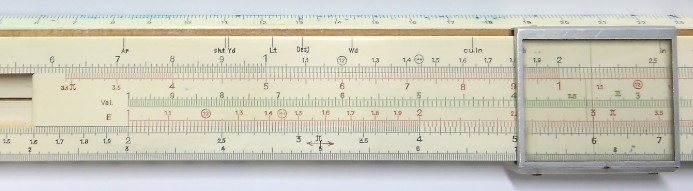
\includegraphics[width=6cm]{SlideRulerScreenshot_2023-12-06_194105.jpg}

对数是计算尺背后的原理。(如果不用计算尺,也可以查对数表得出答案。)

对数是16世纪纳皮尔先生(John Napier 1550 --
1617)用了超过20年时间“发明”的。

\framebox{%
\begin{minipage}[t]{0.97\columnwidth}\raggedright
对数的简单例子:
在草稿纸上就能算出``10,000×100''的结果,同时,我们也可以通过将``10,000''和``100''的``0''相加,得出答案为``1,000,000''。也就是说,把``10,000''看作是"10''的四次方,把``100''看作是``10''的平方,将四次方和平方的4加2,即可得出答案。纳皮尔注意到了这一数字法则,总结出了对数的概念。

计算``10,000×100''的话,使用乘法会更快,但如果数字位数较大,需要手动计算时,使用加法运算会更加简单。纳皮尔先生按照这思路制作出对数表,简化了计算。

看到这里,也许有读者会想``这不就是指数运算的法则吗?''即是说,按照指数运算的法则``\(a^m \times a^n = a^{m+n}\)''来思考的话,\(10,000 \times 100 = 10^4 \times 10^2 = 10^ {4+2} = 10^6 = 1,000,000\),如此便可导出答案。然而,在纳皮尔时代并没有指数这种书写方式,指数的概念也不明确。纳皮尔的伟大之处也正在于此,他在没有指数这一概念的情况下发现了对数,并将其归纳为一个体系。
\strut
\end{minipage}}

可以想象16世纪欧洲,数学研究还是早期,能发现对数把本来复杂耗时的乘或者除变换成log后变成加和减计算本身已经是绝不容易,为了体现这个做法他还单靠个人努力,用了20年时间手工计算出相关对数表。现在我们可以还是可以找到他当时算出的对数表,用现在的计算机验证一下他的8位数头7位还是准确的。

\framebox{%
\begin{minipage}[t]{0.97\columnwidth}\raggedright
纳皮尔先生的对数表: 例如:第一行列出18°30′的正弦值为
0.3173047,对应对数值为 0.111478920。

%\href{文件:微信截图_20230724085408.png}{550px\textbar{}无}
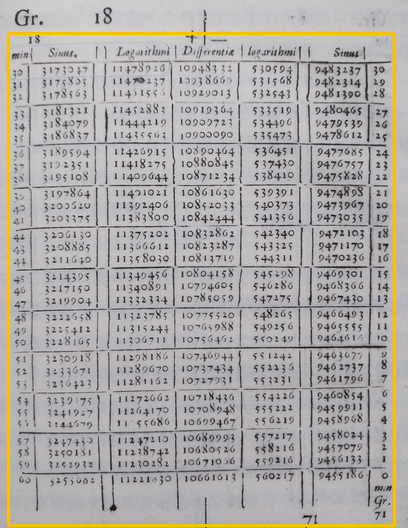
\includegraphics[width=6cm]{微信截图_20230724085408.png}
\strut
\end{minipage}}

纳皮尔先生也研究球面三角学,使用他的纳皮尔公式角度与球面弧(距离)之间关系。
16世纪欧洲国家主要靠航海发现新大陆来发展。但海员在大洋中如何知道自己的位置,船员在大海中只能依赖天上的星星,用六分仪估算船经纬度。使用纳皮尔公式,便能估算A
和B点之间 地球球面弧长。



16世纪欧洲国家主要靠航海发现新大陆来发展。船员在大海中只能依赖天上的星星,用六分仪估算船经纬度,从而知道自己的位置。

纳皮尔先生也研究球面三角学,发现角度与球面弧(距离)之间关系公式如下:

\framebox{%
\begin{minipage}[t]{0.97\columnwidth}\raggedright
\(\cos \theta =  \cos \varphi \mathsf{A} \cos \varphi \mathsf{B} \cos\)(
\(\lambda \mathsf{A}\) - \(\lambda \mathsf{B}\) ) +
\(\sin \varphi \mathsf{A} \sin \varphi \mathsf{B}\)
\strut
\end{minipage}}

海员只要知道两点(A和B)的经纬度(角度)便能使用以上纳皮尔公式,估算A和B点之间地球球面弧长。

例子--北京和巴黎距离:

\begin{description}
\tightlist
\item[]
A: 北京中心位于北纬39°54′20″,东经116°25′29″。 转换为纬度 39.905556, 经度
116.424722。

B: 巴黎转换后纬度48.8583 经度 2.29451。
\end{description}

\framebox{%
\begin{minipage}[t]{0.97\columnwidth}\raggedright
\(\cos \theta =  \cos \varphi \mathsf{A} \cos \varphi \mathsf{B} \cos\)(
\(\lambda \mathsf{A}\) - \(\lambda \mathsf{B}\) ) +
\(\sin \varphi \mathsf{A} \sin \varphi \mathsf{B}\)

\begin{description}
\item[]
\begin{description}
\tightlist
\item[]
=\(\cos 39.905556^\circ \times  \cos48.8583^\circ \times \cos\)(\(116.424722^\circ  - 2.29451^\circ\)
) \(+ \sin 39.905556^\circ \times  \sin48.8583 ^\circ\)
\end{description}
\end{description}

\[= 0.767103 \times 0.657923 \times\](\(-0.40881\))\(+ 0.64152 \times 0.758084\)

\[= 0.28\]

\[\theta = 1.287\] (rad) AB 距离 = 地球的半径
\(6,378KM \times 1.287 = 8,208KM\) (实际距离是 8,217KM)
\strut
\end{minipage}}
当时没有电子计算机,他发明了对数解决这类乘除难题(对数不仅仅用于航海,也帮助天文学计算)。对数帮我们完成复杂计算超过350年,到电子计算器出现才退出舞台。
对数帮我们完成复杂计算超过350年,到电子计算器出现才退出舞台。

\hypertarget{ux521bux65b0-creativity}{%
\subsection{创新 Creativity}\label{ux521bux65b0-creativity}}

不是每个人都能像纳皮尔先生做出创新发明,为人类做出巨大贡献,但他也是普通人,为什么驱动他花20年精力独创对数?

\framebox{%
\begin{minipage}[t]{0.97\columnwidth}\raggedright
Robert Fritz 回忆:``60年代,当我在Boston Conservatory
学音乐作曲时,开始思考学的不应仅仅是对位、和音,更要了解音乐大师们的创新过程。''\\
他毕业后继续做音乐创作,一次参加创新专业人士聚会,包括作家、画家、音乐家、建筑师等,他发现这些人在针对本身专业的创作能力都很厉害,但都没有想到用他们的创新能力提升自己的生活。

他便开始举办培训课帮不同背景的人提升创新,让各个行业也可以学什么是创作/创新。几年后,他把创作的重点写成了一本书
(见 Reference 参考)。Robert Fritz 在他的书中,以贝多芬为例,说明创作并非
Problem
Solving(解决问题),而是要有很高的目标/理想,然后不断地尝试比较,最终达到创作目的。
\strut
\end{minipage}}

\hypertarget{ux521bux9020ux7684ux7cbeux795e-spirit-of-creating}{%
\subsection{创造的精神 Spirit of
Creating}\label{ux521bux9020ux7684ux7cbeux795e-spirit-of-creating}}

创作不是由他人驱使,而是出于自身创作的欲望,要创作世界上最优秀的作品。觉得自己的创作很有价值,会用尽精力努力创作,最终希望自己的作品以后有自己的生命力,受他人赞赏。

伟大的创新者不仅仅要有与众不同的目标,更要有超凡的能力和巨大魄力,才能对以后人类的发展作出重大影响。

贝多芬追求完美,拥有极大的魄力,不断完善,才取得超人成就。

贝多芬对音乐创作的远景目标 ------
希望创造前所未有的作品(他觉得当代的作品,甚至包括他老师海顿和音乐天才莫扎特的作品,离这远景还差很远)。由这崇高的目标驱动,加上他自身的音乐演奏和作曲能力,不断突破,甚至耳聋也阻挡不了他的创作力(从25岁开始听力减退,到45岁已经完全失聪),让音乐创作升一大台阶,深远影响以后的作曲家。\\
%\url{文件:Bdf.png}

%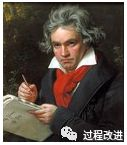
\includegraphics[width=6cm]{Bdf.png}

\framebox{%
\begin{minipage}[t]{0.97\columnwidth}\raggedright
\textbf{贝多芬} (1770 --
1827)的音乐创新可以说是前无古人后无来者,深深影响着后面两个世纪的作曲家。\\
我们都熟识他的命运交响曲,其实他从1795年到1827年去世前出版的每一首作品,无论是交响曲、室内乐
或
歌剧,都是经典。他是完美主义者,例如《田园交响曲》的创作时间不少于3年,从他手稿得知,首乐章某主题他修改了不下12次,所以与巴赫,莫扎特,舒伯特比较,他的``生产率''不算高,平均每年出版5\textasciitilde{}6个作品。

他出版《命运交响曲》、《田园交响曲》时(1808),已经出版音乐作品13年,包括23首钢琴奏鸣曲,9首弦乐四重奏。
开始时,作品类似海顿、莫扎特的风格,但是到了中期,如《命运交响曲》、《田园交响曲》,已经远远超出他的前辈和同辈,启蒙音乐家从古典期发展成浪漫期新风格。

例如,低音大提琴
一直在乐队里只担当伴奏角色,在命运交响曲第三乐章,贝多芬让低音大提琴先弹出轻快的主题后,大提琴接棒演奏同一主题,之后让中提琴接棒,最后又小提琴接棒。这种交响曲风格是前所未有。(他写作时,还特意咨询当代杰出低音大提琴师
Dragonetti,咨询他技术上是否太难,是否超出乐手的能力。))

例如,第九交响曲,在最后第四乐章加入四声与合唱(传统交响曲只有乐队演奏)。

晚期的作品(如钢琴曲、弦乐四重奏等),又呈现出与中前期不同的另一种风格。例如他的Op133
弦乐四重奏 Große Fuge
由于思路远超于当时的水平,不被当时的音乐家接受,觉得作品有问题,有些甚至说他太老,止聋了还疯了。但贝多芬依然故我,说``这曲是为未来写的!''

他的音乐创作一直没有停下来,例如他的最后弦乐四重奏(第16首)Op135在1826年出版。

\strut
\end{minipage}}


\framebox{%
\begin{minipage}[t]{0.97\columnwidth}\raggedright
贝多芬 一生写了32首钢琴奏鸣曲 ,与莫扎特和他老师海顿不同,贝多芬每一首钢琴奏鸣曲虽然都是奏鸣曲式,但都有独特创新,突破奏鸣曲式,变化万千。

赋格曲 (Fugue)(\#)从16~17世纪不断演变,到了18世纪,
J.S.巴赫把这曲式创作提到巅峰,例如,他著名的《平均律钢琴曲集》 The
Well-Tempered Clavier Book I \& II (BWV 846-893),
共两本书,每一本书,从C大调一直到B小调,共24 首前奏与赋格(Prelude and
Fugue),是赋格曲创作的典范。

贝多芬在晚期作品中有很多基于赋格曲的创新,例如
他的第29降B大调钢琴奏鸣曲(Hammerklavier Op.
106)的最后第四乐章便使用赋格曲曲式。
虽然他使用了赋格曲的各种技巧,如不同的速度、上下颠倒、从后往前等,
但他不会完全像巴赫,严格按照规定,让听众觉得虽然听起来是赋格曲曲式,但又好像不同于传统赋格曲,有全新的感觉。
整个第四乐章超过12分钟(巴赫《平均律钢琴曲集》里的赋格曲大多是两三分钟,最长才6\textasciitilde{}7分钟
)。
整个奏鸣曲长达接近45分钟,还有很多其他前所未有的创新,把西方音乐创作提升一个台阶。

(\#)
赋格的特征:开始时,第一声部单独唱出第一主题,然后,第二声部或移高五度或降低四度进入,然后,第三声部进入,一直到最后声部。每个声部进入后会继续唱,各声部也要满足和声和对位法的要求。各声部都进入后,
第一声部会唱出第二主题,其他声部也会轮流进入。
\strut
\end{minipage}}

Fritz
发现这些大师有共同特点:把握自己命运,追求个人目标的主动心态。很多人也很有才华,为什么他们大多数都不能成为大师?他用下图解释。除了要对未来有远景目标外,了解现状同样重要。如果不觉得有差距(张力),就没有改进的驱动动力;有些人有理想,但缺乏计划与行动,便只是梦想。

%\href{文件:liuct.png}{600px}

\includegraphics[width=6cm]{liuct.png}


这创新动力模型不仅仅适用于音乐创作。例如纳皮尔先生为了解决正弦相乘的困难,发现可以换成对数,使乘简化为加 (VISION),为了可应用,还花了毕生精力计算对数表 ,也是从张力,化为行动(ACTION)并创新的例子。



\hypertarget{ux516cux53f8ux5982ux4f55ux521bux65b0}{%
\subsection{公司如何创新}\label{ux516cux53f8ux5982ux4f55ux521bux65b0}}

\framebox{%
\begin{minipage}[t]{0.97\columnwidth}\raggedright
这公司创作的产品在你身边的人中有大于50\%
机会都有使用,包括各种年纪,公司产品功能广泛,包括听音乐、打电话、电脑/平板、网上看视频和日常工作。请你猜猜公司名?
\strut
\end{minipage}}

苹果公司 (Apple)

我和全世界千千万万人一样每天都在使用苹果产品:iPhone、iPAD平板电脑和iTune网上搜索音乐歌曲,要了解苹果的成就,便不能不谈乔布斯
(Steve Jobs)。他一生充满传奇,很多故事,可读"Steve
Jobs"一书了解。让我们先回顾苹果如何成为大众音乐市场巨人的故事。

\begin{description}
\item[]
\begin{description}
\tightlist
\item[]
= = =
\end{description}
\end{description}

\hypertarget{ux97f3ux4e50ux64adux653eux5668}{%
\subsection{音乐播放器}\label{ux97f3ux4e50ux64adux653eux5668}}

80年代末开始出现MP3格式,可以把歌曲数据化,市场开始有一些可以随身携带听音乐的小设备,但因为技术有限,都不理想,乔布斯本身也很喜欢音乐,就看准这市场,希望把苹果电脑定位为个人各种电子设备(包括音乐播放器)的集合点(Hub)。首先要解决播放器方便携带,容量够多。当时还没有合适的小型显示器,锂电池和小硬盘。过了几个月开始找到合适,例如东芝刚研发出一款超小的5G硬盘,只一英寸直径,像个大银币。他们比较当时市场常用的播放器,发现都不好用。容量也不足,也难以按自己喜好排列歌曲顺序,如果要从CD把歌曲下载到电脑,并要按自己喜欢的顺序来让播放器去播放,其实是挺复杂的过程。但是如果把那些功能都放在播放器操作,但播放器屏幕小,太困难了。
他一直非常关注产品易用性,内部软件研发工程师首次展示正开发中的刻录软件,乔布斯听完他们展示后,就站到白板上画了一个框,说“你们设计软件就是要把歌曲拉到那个框里面,点击一个按钮刻录就行了。”当时软件工程师被吓呆了,觉得很难做到,但工程师往往不会从用户的视角看问题。所以后面乔布斯要求播放器的软件都需要给不懂技术的人使用,让她可以在3个步骤内,不用看说明书,完成任务,这是他的测试要求,做不了他不会接受开发出来的软件。播放器设计也要创新,比如用家可以滑动面板的轮来选歌,他只要在这轮不断的滑动就可以跳到要选的歌曲,很方便。iPod也体现了苹果设计的概念——简洁。产品的设计选择白色,包括耳机也要白色(当时,大部分耳机都是黑色),还有连充电器整也是白色。设计师Jony Ive 解释:“白色可以让他觉得这个产品很高贵,跟那些其他廉价的播放器有极大的区分,会觉得设计有艺术感。”


%\href{文件:R-C_(2)_副本.jpg}{350px}

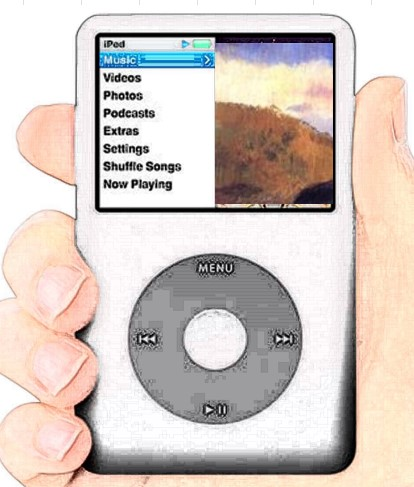
\includegraphics[width=6cm]{!ipodcutoutScreenshot_2023-12-06_201652.jpg}

乔布斯也非常注重产品包装,iPod的包装让你觉得:``在拆包装时,觉得有一件很贵重的东西在里面''。

%\href{文件:IpodPackageScreenshot_2023-07-23_201312_labi.jpg}{400px\textbar{}无}

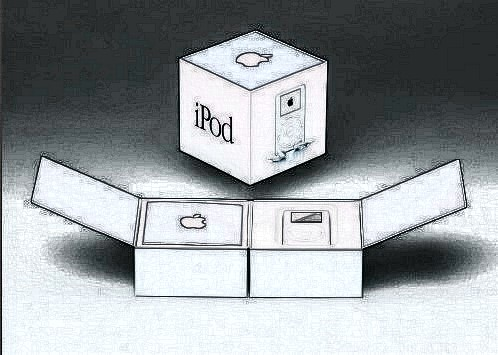
\includegraphics[width=6cm]{IpodPackageScreenshot_2023-07-23_201312_labi.jpg}

虽然定价不低:399美元,很多人觉得定价过高,但是iPod在2002年正式推出市场后一直热卖。

\begin{description}
\tightlist
\item[]
= = = =
\end{description}

从2001年到2014年苹果大概卖出了4亿件iPod,2015年后还继续卖出50,000,000件。iPod播放器也成为了苹果的主要收入来源。2006年是苹果推出iPhone前一年,iPod销售占公司总收入的40%。下图展示了从2002到2013年,iPod的销售数量变化(柱形)和收入占比变化(曲线):

%\href{文件:IPodRiseFallScreenshot_2023-07-22_164335.jpg}{300px}

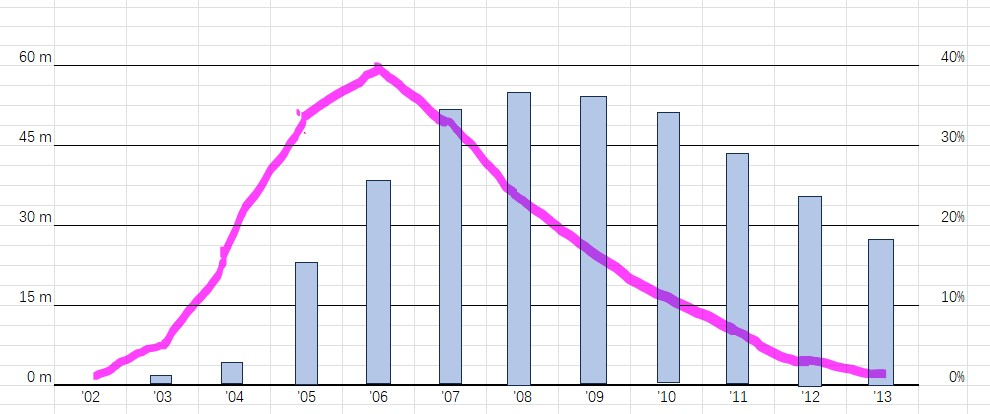
\includegraphics[width=6cm]{AppleRiseFallDrawScreenshot_2023-12-06_211749.jpg}

\hypertarget{itunes-ux7f51ux4e0aux5546ux5e97}{%
\subsection{iTunes 网上商店}\label{itunes-ux7f51ux4e0aux5546ux5e97}}

苹果的iPod加上Mac机里的iTune应用软件很成功,但只解决了可以从网上下载音乐在手提播放器听歌的技术问题,但有更严重的问题要解决——盗版,2000年开始,越来越多网站提供免费音乐下载,大大影响了唱片销售(2002年销售额就跌了9%),也侵犯了音乐歌曲创作者的知识产权保障,各唱片公司都急于解决这冲击,但大部分唱片公司都没有技术能力创建自己的网上平台。乔布斯也很看重这些创作人的利益,他可以预见到如果没有知识产权的保障,就没有人再有动力录制高质量的歌曲和作品(如果软件与电脑没有知识产权保障,就没有公司愿意投资做创新)。

所以他就基于iPod和iTune能结合音乐播放与电脑的功能,开始展示给各大唱片商网上平台如何运作,如何防止盗版,因唱片商都缺相关的技术能力,很快便有4家唱片商有兴趣并愿意合作,利用iPod、iTune等技术,筹办统一平台服务,让消费大众可以在网上购买并下载歌曲。

从2002年开始,乔布斯一直忙于周旋各类问题,除了技术方面格式问题要解决,例如各有自己的格式,要统一,还有,唱片商都想保护自己的利益。比如索尼,因自身的技术能力也很强,也想自己建立平台(索尼最终未能成功,本章后面会细说)。

最终在2003年4月,iTunes store 正式推出市场,大家可以在网上用关键字搜索任何一家唱片公司的唱片或歌曲,也可以搜索相关的唱片。乔布斯的业务模式很简单,他从以前的经验知道首先要廉价,让大批的人群进入使用。如果收费太高,只是小部分人使用,就流行不起来,也没有动力吸引新唱片公司加入,恶性循环。他的策略很成功。

2003年苹果刚开始发布iTunes 网上商店时有200,000歌曲可以下载购买。本来预测这新服务可在6个月内销售100万首歌曲,但实际上推出6天就已经卖了100万,2003年12月累积卖出2500万首歌曲。

2004年7月份共卖出一亿首歌曲(2003年底的4倍);2005年11月(两年半后)苹果成为全美国十大音乐零售商之一,其他都是传统零售商,例如第一是Walmart。

随着网上买歌商业模式越来越普遍,传统零售商越来越困难,到了2010年2月,苹果成为美国最大的音乐零售商。

今天,因为网络技术发达,不再是当年的网上下载,但很多人还是喜欢只须要每个月交几十块钱就可以随时随意在网上搜索并听到自己心爱的歌曲,这商业模式也保护了艺术家、唱片公司的利益。

\hypertarget{ux516cux53f8ux5982ux4f55ux521bux65b0-1}{%
\subsection{公司如何创新}\label{ux516cux53f8ux5982ux4f55ux521bux65b0-1}}

从以上乔布斯关于音乐的故事,可以看到跟400年前不一样,400年前纳皮尔的创新前后要20年,速度很慢,靠一个人独创。帮了人类进了一大步。到了2000年什么速度都变快了,乔布斯团队经过3个月就推出iPod播放器,也同时间用了两年时间,创建了 iTunes 网上音乐平台,保护了艺术家、唱片公司,软硬件设备供应商各方面的利益,也帮苹果公司定位成数字中心(Digital Hub),消费者可以使用电脑选择喜爱的歌曲在iPod 播放,也可以下载最新的歌曲,非常方便。这些就是我们2000年代看到的创新,这些创新不可能靠一个人独自完成,而是要团队合作。

公司创新与几百年前那些大师的创新最大的区分是需要整个公司所有人的协作,大家目标也要一致。整个系统都要都要配合,但是不同人负责执行不同的工作,所以目标要细分。

纳皮尔先生用了20年,写了3本数学书(一本是他死后出版),总共不到200页。贝多芬生产率也不高,一年出版几首作品,这些大师都是靠自己一人完成整个创作。但是现代市场变化越来越快,要成功,公司必须快人一步,但因依赖团队合作(各有专长),也需要协调大家的工作,确保各个层次的目标与公司总目标一致。

举例介绍企业如何用一个简单系统来管理整个公司的提升:

\begin{enumerate}
\tightlist
\item
  识别公司的总目标

  \begin{description}
  \tightlist
  \item[]
  例如在下一年,要一年内生产7个新的产品系统。
  \end{description}
\item
  描述公司的现状

  \begin{description}
  \tightlist
  \item[]
  例如现状是:平均一年只能产出3个新产品,有2个开发团队。但开发人员的能力有限,质量也不好,导致用了不少精力,去维护已经完成的产品,没有时间来开发新的,招新人也不容易,比较难找得合适的,也没有时间培养新人,扩大工作。
  \end{description}
\item
  形成具体行动计划

  \begin{description}
  \tightlist
  \item[]
  例如简洁、清减的开发流程,增加1个开发团队,加强代码评审和编码能力,来减少缺陷导致的返工,要跟市场部密切合作,确保新产品满足客户的要求,给客户带来价值。

  但真正公司的从上而下总计划会更具体。
  \end{description}
\item
  当我们定好明确的最终结果,也了解真正的现状,有一些行动计划,下一步是具体到每活动的完成日期和负责人。
\end{enumerate}

%\href{文件:Fritz_diagrams_3.jpg}{550px}

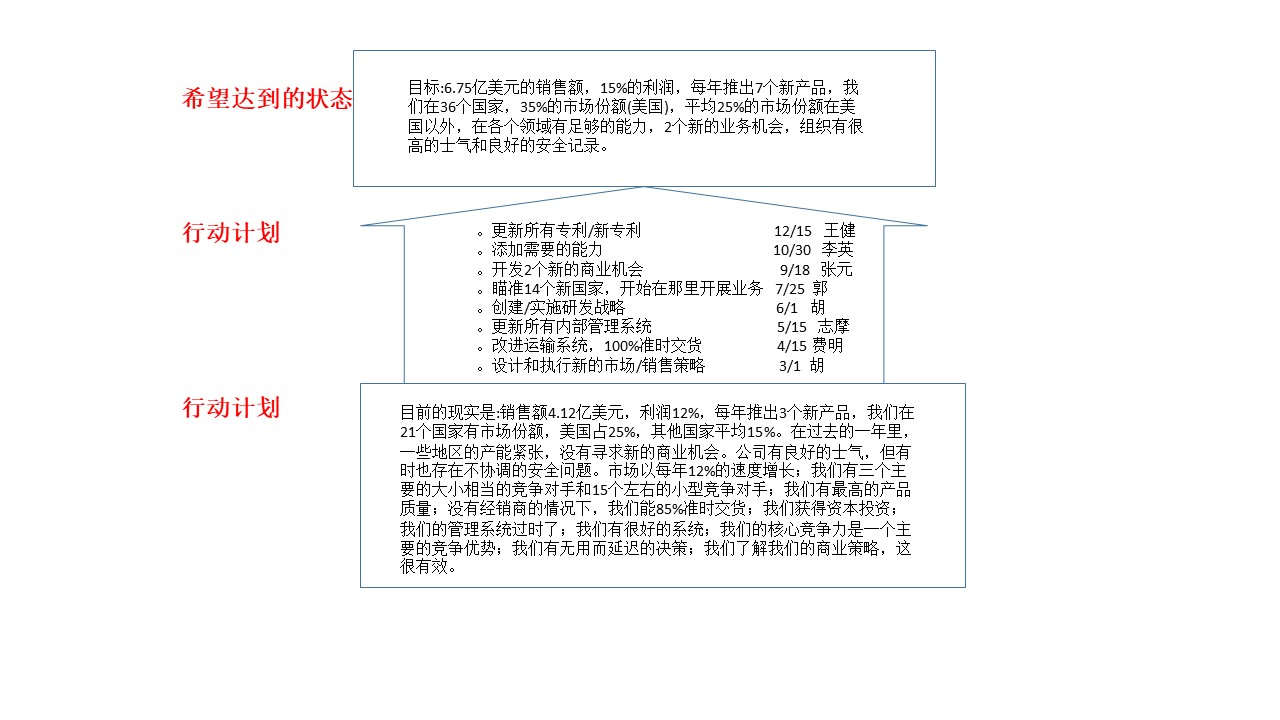
\includegraphics[width=6cm]{Fritz_diagrams_3.jpg}

同意可以用以上模式帮助公司创新吗?
请看看乔布斯另外两个公司创新故事(非苹果公司),你可能有不同想法。

\hypertarget{ux4e07ux4e8bux8d77ux5934ux96be}{%
\subsection{万事起头难}\label{ux4e07ux4e8bux8d77ux5934ux96be}}

乔布斯1985年9月被迫离开苹果公司后,自己投资700万美金,独力开创一家专门针对高校工作站市场的新公司 NeXT。乔布斯开始时对公司的期望特别高,当时他看到这市场主要被太阳(SUN) 和(DEC) 公司占有,但这些工作站产品都是以输入命令为主,与Macintosh用鼠标操作不同,所以易用性不高,所以他希望创造前所未有的新平台,让那些高校的学者与研究人员可以简单地使用电脑模拟各种场景来做研究。

但是要达到这么高的理想,要做的工作就非常多。比如第一次公司开创90天后就开始有一次度假村的头脑风暴会议,希望可以在两年后推出产品,赶上学校暑假购买的时期,再过了3个月,再讨论时,大家都发现这个要求太高,难以实现。但乔布斯没有放弃,他一直用自己的魅力说我们可以按大家的专长达到这个目标。

1986年过去,1987年又过去了,一直都没有把新产品研发出来。到了1988年开始做了第一次3个小时的产品演示,但产品还是很初级,例如都没有颜色,速度也比较慢,虽然签了以前为苹果推销Mac的全国电脑零售商,但一年才卖了360台,离目标差很远。(1984年,那家全国零售商一年就为苹果卖了40万部Mac;NeXT工厂生产线是按每月生产1000台做设计规范!)

1990年,第2次产品发布,新产品开始有了颜色,速度也提升了。但是还只算是初级产品,未成熟。

因销售不理想,乔布斯再增加了500万投资,很快也用光。幸好有一位外部投资者 --- 德州企业家 Ross Perot 先生,他非常相信乔布斯的魅力(他觉得以前没有来得及投资他的苹果,一直耿耿于怀),他投资了2000万美元进NeXT。但因为这操作系统被苹果看中,NeXT公司最终于1996年被苹果公司用43千万美金收购,也让乔布斯重返苹果公司(开始时当顾问),经过15年努力,使苹果公司再创辉煌。

到1993年开始裁员。公司开始本来有600人,开始只是裁几十人,后面再裁员200多人,接近公司的一半人数,后面又裁200多人,最终把整个硬件部分卖掉给日本佳能公司,只保留操作系统部分NextStep。

\hypertarget{ux4eceux5febux7834ux4ea7ux53d8ux4e3aux6295ux8d44ux56deux62a5ux6700ux597dux7684ux6295ux8d44}{%
\subsection{从快破产变为投资回报最好的投资}\label{ux4eceux5febux7834ux4ea7ux53d8ux4e3aux6295ux8d44ux56deux62a5ux6700ux597dux7684ux6295ux8d44}}

乔布斯在1986年用一千万美元投资Pixar(“公司”本来是 LucasFilm 下属30多人的电脑部,由《星球大战》导演George Lucas 投资创立,主要支撑电影的动漫效果需求;因为乔布斯一直对美术很有兴趣,他经Alan Kay介绍去公司看展示便被这公司的产品深深吸引,觉得很领先,远远超前同行);乔布斯开始时只是投资者,没有太干预,公司的软硬件产品,针对高端动漫专业人士使用,但他雄心勃勃,觉得产品很有特长,希望和苹果Mac一样大量,买给做动漫人士使用,做3D设计。例如产品虽然功能很强,但都需要复杂的命令操作,不适合一般动漫人士使用(但其他如Adobe公司的软件,虽然功能没有这么强,但很容易用),便投入研发,希望改善不足;为了推销全国,他还开始开零售商店。

乔布斯对公司的投入投资也越来越大,但产品销售一直没有起色,公司开始缺乏资金,1988年他开始紧束开支和裁员。直到1991年,与迪士尼合作Toy Story,使Pixar起死回生,乔布斯共已投入了5千万美元(占他从苹果公司股票卖出股票收入的一半)。也因与迪士尼成功合作,让Pixar能在1995年(与Toy Story首次公演同年)挂牌上市,为公司取得15亿美金投资。Pixar与迪士尼继续合作,推出5部电脑制作动画,都非常卖座,于2006年,迪士尼为了防止Pixar与其它公司合作,用74亿美金收购Pixar,也使乔布斯成了迪士尼的最大独立股东。(关于Pixar Toy Story制作故事,请看附件)

\framebox{%
\begin{minipage}[t]{0.97\columnwidth}\raggedright
后面事实证明乔布斯以为一般动漫人士会喜欢用Pixar的3D模型软件是错误的,只是梦想。但他的另一个希望:如何结合电脑数字技术和艺术做创新,确能梦想成真,Pixar与迪士尼合作制作新一代动漫片,从1995年的Toy Story开始,把动画片技术提升一个台阶。

%NeXT:本来希望大量生产高校用的工作站电脑,与太阳SUN DEC竞争,最终经过多年的努力,只卖出几百台,为了生存裁员和把硬件部分全部卖给佳能公司,只留下操作系统NextStep。但因为这操作系统被苹果看中,NeXT公司最终于1996年被苹果公司用43千万美金收购,也让乔布斯重返苹果公司(开始时当顾问),经过15年努力,使苹果公司再创辉煌。
\strut
\end{minipage}}

从上面两个故事看到企业创新都会经历原本预料以外的环境。
所以任何创业公司因为市场是未知,有超过90\%的创新产品都可能以失败告终,所以无法用以上传统的企业策划方式。也验证了马云先生的名言``今天很残酷,明天更残酷,后天会很美好,但绝大多数人都死在明天晚上''。

\hypertarget{ux516cux53f8ux521bux65b0ux6210ux529fux8981ux7d20}{%
\subsection{公司创新成功要素}\label{ux516cux53f8ux521bux65b0ux6210ux529fux8981ux7d20}}

回看iTunes电子商店的和之前iPod的成功故事,和乔布斯之前的NeXT和Pixar故事,可总结以下成功要素/注意事项:

\hypertarget{ux7075ux6d3bux654fux6377}{%
\subsubsection{灵活、敏捷}\label{ux7075ux6d3bux654fux6377}}

从物种进化历史可以看到物种可持续的原则:

\begin{itemize}
\tightlist
\item
  最强壮/巨大的物种也会灭绝(如猛犸象)
\item
  最凶猛的物种也会面临灭绝(如狮子、老虎)
\item
  只有最能快速适应环境变化的物种才能长期传承下去
\end{itemize}

从60年代开始,商业环境快速变化,也只有能快速适应环境的公司,不断求变,才能持久,成为百年老店。

从乔布斯的NeXT和Pixar故事看到,要创建一些新的产品服务变数很多,失败机会很大。所以要随时变招适应变化。如果发现本来的想法、计划没有成果,就立马要改变。

这道理适用于很多科技公司,比如谷歌也有很多失败的项目,谷歌的宗旨是'Fail
Fast'
,项目如果过了半年,九个月。没能达到一定的客户量,就会立马叫停,终止这个项目。很多科技公司都是年底,才综合考虑某业务是否持续,可能已经太慢了。

这也是敏捷开发的原则:不花精力于长远的策划中。因为需求常常变化,分成小迭代,每迭代冲刺,基于有限资源,尽力把每次迭代做好:不仅仅效率高,产品质量也要好。

\hypertarget{ux4e13ux6ce8focus}{%
\subsubsection{专注(Focus)}\label{ux4e13ux6ce8focus}}

资源有限,只关注公司自己能做好的东西,哪些可以外包,就尽量外包。比如生产,苹果只专注做好自己的专长
- 产品设计。(请不要误会苹果不管生产,它的产品生产都是按JIT做,
只是非直接聘用生产工人。)

乔布斯回到苹果后,吸收了过去十年在NeXT 和 Pixar
的经验教训,本来苹果公司里面一百多个研发项目,乔布斯很了解资源有限,便开始整合,只留下每个市场最好的研发项目,解散不需要的研发团队,只留下跟公司发展愿景相关的研发。

乔布斯2010年被访问时说:``我们选技术,只挑选有发展潜力的技术,保全宝贵资源,因什么都支持,都研究就会耗费宝贵资源。''

\hypertarget{aux7ea7ux56e2ux961fux6210ux5458}{%
\subsubsection{A级团队成员}\label{aux7ea7ux56e2ux961fux6210ux5458}}

Pixar公司虽然小,但每位都是行业精英。

\framebox{%
\begin{minipage}[t]{0.97\columnwidth}\raggedright
我美国堂弟从小很喜欢动画人物,家里全都是星际旅行、星球大战等模型。他来香港旅游也专门去那些小的专门店找他喜欢的卡通人物模型。他读建筑专业毕业后专攻动画片和主题乐园设计。
他和其他3位设计师是公司外聘参加超人总动员》制作设计的原始核心团队。其他3位都是行业中的有名高手,例如,Blackman
曾设计蝙蝠侠系列,Delgado 设计星际旅行(Star Trek)等。

他说``Pixar公司在动画片行业非常出名。
核心制作团队,包括艺术总监和生产设计师等都是当时行业的顶尖高手,
他们除了能力超强,对艺术创作的品味与兴趣跟我也很相似,能有这机会与他们共事合作
真是非常幸运,像中了彩票一样。开始时,我们四位设计主要成员定期要跟导演Brad
Bird 开会,评审设计。``
超人总动员》非常卖座,美国本土票房收入已经超过2亿美元,也得了奥斯卡奖。

Pixar公司这些动画片,能有这么好的票房,并得奖,不是没有原因的,因为公司有名气,可以吸引到当时最优秀的艺术家参加,有了这些人,我们才可以看到像《超人总动员》这档次的高端制作。
\strut
\end{minipage}}

所以当A级成员遇上能力相当的团队伙伴,更能擦出火花, 1+1 大于 2 的效果。

苹果公司1984年发布的Macintosh,产品的技术能力和设计(例如,视窗,鼠标等)都远远超越了之前IBM出的IBM PC。开发团队成员的能力超强,里面包括 Burrell Smith设计硬件线路版,Andy Hertzfeld 等设计Mac GUI 操作系统, Bill Atkinson设计Graphics应用软件QuickDraw, HyperCard,Joanna Hoffman 负责市场推广,Bruce Horn设计Resource Manager 应用软件等。但产品发布后,因为销售不太好,管理层也换了人,团队成员都陆续离开。

乔布斯从Pixar的经验,深明高端球员(A
Players)只愿意与高端球员搭档的道理。但为了吸引和留住这些精英,公司必须给有吸引力的报酬。

例如,乔回苹果不久就特别要求董事会修订员工股权安排(因当时苹果股价已经很低,之前的员工股权安排已经没有意义。)

\hypertarget{ux6781ux9ad8ux76eeux6807ux8981ux505aux5927ux505aux5f3a}{%
\subsubsection{极高目标,要做大做强}\label{ux6781ux9ad8ux76eeux6807ux8981ux505aux5927ux505aux5f3a}}

\framebox{%
\begin{minipage}[t]{0.97\columnwidth}\raggedright
在杭州某商务酒店看到十几条浙商名言,写在墙上,其中一条如下:

%\href{文件:mingyant.png}{600px}
\includegraphics[width=6cm]{mingyant.png}
\strut
\end{minipage}}

乔布斯创立NeXT时是世界第一的工作站供应商,所以生产线是按每月能生产一千台设计!
他重回苹果后,也一直按做出世界第一产品推动团队,后面事实证明 ,例如 iPod
/ iTunes(2001) , iPhone(2007),
iPad(2010),这思路使苹果公司后面成为美国市值最大的科技公司。

丰田大野耐一 说过, ``容易达成的目标不是好目标''
,他对丰田员工设的质量目标是零缺陷!

\hypertarget{ux6709ux975eux5e38ux9ad8ux7684ux8981ux6c42ux7528ux5fc3ux505a}{%
\subsubsection{有非常高的要求,用心做}\label{ux6709ux975eux5e38ux9ad8ux7684ux8981ux6c42ux7528ux5fc3ux505a}}

每位团队成员都有高度的要求,不仅仅是做完事,要做出优秀的、世界一流的产品,有这种抱负才可以驱动每一个人辛辛苦苦付出最大努力把这件事做好。例如乔布斯自己就是典型例子,他信心这些是有价值所就全心去做好。比如在推出iTunes电子商店以前他就不断的邀请各种音乐家、歌手、音去家。他每次都会想尽办法去介绍他的好东西,有一次小号手W. Marsalis到家拜访,乔布斯就问他:“你喜欢什么歌曲?”

Marsalis
说:``贝多芬'',他就一起展示如何在商店里面可以容易搜索到,Marsalis后面回顾说:``其实我一直都不太对电脑感兴趣,但乔布斯他一直全心全意,全程用了两个小时很细心地给我介绍。过了一会,我的注意力不是放在他的产品或者电脑上,而是他本人,我深深被他的激情/专注打动。''

例如苹果的首席设计师 Jony Ive
用简洁设计思路,让消费者觉得苹果产品有艺术感,非一般电脑:

%\href{文件:Power_Mac_Screenshot_2023-07-05_131914_副本.jpg}{300px}

%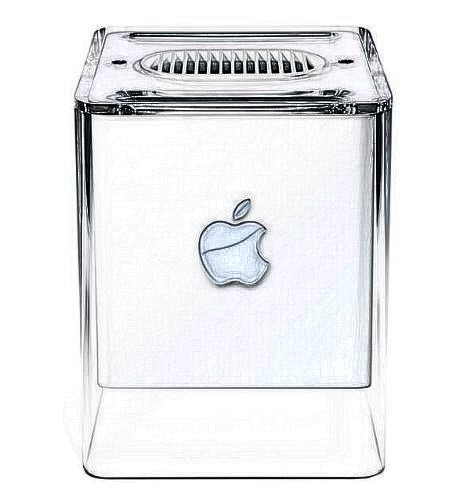
\includegraphics[width=6cm]{Power_Mac_Screenshot_2023-07-05_131914_副本.jpg}

%\href{文件:R-C_副本.jpg}{300px}

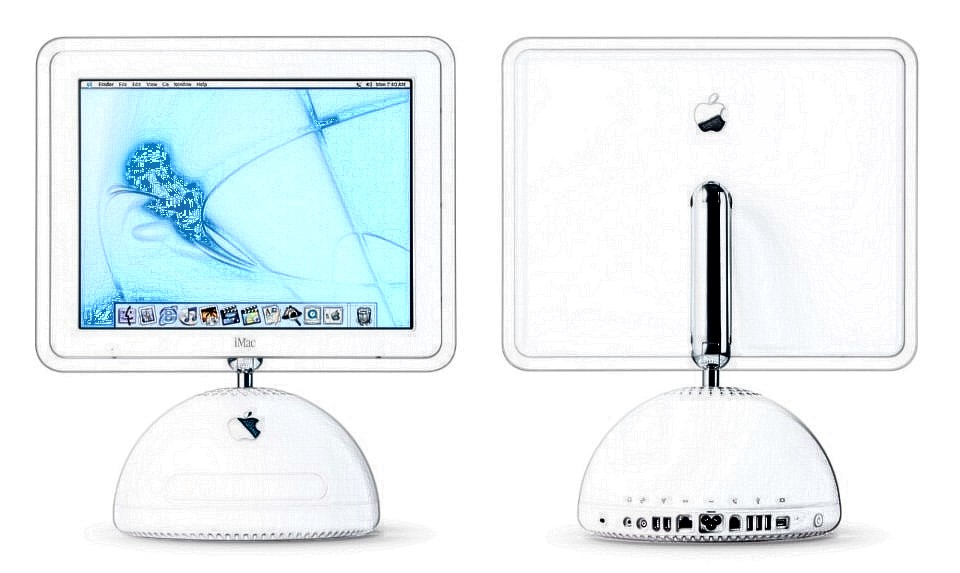
\includegraphics[width=6cm]{R-C_副本.jpg}

Ive的父亲是位优秀工匠,从父亲他学到要做一流工匠必须对质量有极高要求。

\hypertarget{ux9886ux5bfcux51b3ux7b56ux5febux901fux884cux52a8}{%
\subsubsection{领导决策、快速行动}\label{ux9886ux5bfcux51b3ux7b56ux5febux901fux884cux52a8}}

索尼一直在电子产品很有创新,例如Walkman,也有唱片公司;创建网上音乐平台的主要元素它全部都有,但是为什么索尼做不出来,还是让苹果成功。其中一个最大原因是索尼是大公司,由各个事业部门组成,每个事业部要管自己的盈利,也正是这个原因,需要各团队之间紧密协作,很多精力就耗在内耗于内部部门之间的协商,所以最终失败。反过来,苹果是不会这样细分,只算整个公司的毛利,不会细分到每个事业部,而且乔布斯有非常高的要求。例如整个IPod时候的设计,当工程部和软件开发部做了那些原型初稿30个,然后乔布斯进来以后大家都同意这个款式,就基本上立马行动去做了。(有些在其他大公司,比如飞利浦,工作过的员工会觉得很奇怪,因为像西门子、飞利浦那种传统大公司绝对不会在一个会议里做这么重大的设计决策。)

\hypertarget{ux7ed3ux675fux8bed}{%
\subsection{结束语}\label{ux7ed3ux675fux8bed}}

苹果的例子可以看成是敏捷开发升级到公司级的最佳实践案例实例,从前面的故事看到整个公司都是按精益的思路不断改善。

团队合作性很重要,团队的能力要求也很高,才可以在最短的时间做到最好。强调岗位之间的互相合作,不是你是做测试,我是做开发,你是做需求我只管做好自己的工作,必须大家相互合作,最终希望整个项目产品成功,不计较是否在我的工作范围之内,也确保相互是打通的,你自己需求或者开发最优,不表示最后产品可以做到最优,有些开发团队抱怨:“我其实开发挺不错的,但是需求一塌糊涂,我们无法做好。”

但是也因为公司架构原因,部门之间各有自己的领导,自己的指标,导致功能之间不能相互合作做好。

从乔布斯故事了解高层有高度的要求很重要,要做好敏捷开发的一样。如果敏捷团队不注重产品质量,只关注按时交付,最后只能做出一些烂产品;但反过来,当团队有能力,大家有抱负有要求,敏捷开发可以帮助团队快速反应不断变化的需求,像苹果与乔布斯一样成功,世界第一。

1983 ~ 
84年,乔布斯(28岁)在苹果公司带领Mackintosh开发团队时,就不会向预计交付期限低头。如果他觉得产品未达到质量要求,他宁愿延后。他甚至鼓励团员要精益求精。(千万不要以为你在他管理的团队可以偷懒)

有人问我:听过SAFe这个框架吗?我们想用它在公司级推敏捷,你觉得怎么样?
我:框架只是框架,如果你没有我们刚才说那些要素,什么框架都帮不了你。因为那些框架只是把一些最佳实践的要素列出来,有了那些过程,有了一些度量,没有合适的人,没有合适的领导,没有苹果这种公司文化,永远不会做到世界一流的产品。这道理国内外同样适用。

\begin{description}
\tightlist
\item[]
= = =
\end{description}

2005年,乔布斯获史丹福大学颁授荣誉学位,他在典礼中跟其他毕业生讲了三个故事:\\
\textbf{故事一}:\\
高中毕业后,我17岁进了私立的里德大学,学费昂贵。读了半年,我一方面觉得学非所用,另一方面不忍心花掉父母一辈子的积蓄,就退了学。但我并没有离开学校,而继续在学校里旁听感兴趣的课。我没有收入,就睡在同学宿舍地板上,同时靠捡玻璃瓶、可乐罐挣点小钱糊口。因平日吃不饱,每个星期天,我走路到距离七英里的一所印度寺庙去吃一顿施舍饭。

大学的美术字(Calligraphy)课程很有名,我去旁听,立马迷上了。虽然当时我还不知道以后有什么用,但是后来在设计苹果的麦金托什(Macintosh)计算机时,想到当年在大学里旁听的课程,为Macintosh个人电脑设计了很漂亮的字体。

十年后回看,这些生命中的小点都能连起来,但不可能之前预计会连起来,只能事后回顾能看到。所以我们必须相信这些小点会在生命中某时候能连接起来,才有信心按自己信念勇往直前。\\

\textbf{故事二}:\\
我在30岁的时候被苹果公司赶了出来,觉得很失败,没有面子,对不起那些其他创业者。后面因为我还是对电脑IT很有兴趣,我就自己开公司继续做产品研究专门针对工作站希望开发一些世界一流的产品,我现在回想看如果当时没有离开苹果,继续在苹果的话,后面就体验出很多我产品的开发的概念。所以我现在回想过来,一点都没有后悔。最重要就是你必须要热情的爱上,无论是工作或者找伴侣都是一样道理。

“有些时候,生活会拿起一块砖头向你的脑袋上猛拍一下,不要因此失去信仰。我很清楚,支撑我一路走下去的,是那些我所爱的东西。你需要找到你的所爱,工作如此,爱人也是如此。你的工作将会占据生活中很大的一部分。你要相信这份工作是伟大的,你必须先热爱它;你只有坚信自己所做的是份伟大的工作,才能怡然自得。如果你现在还没有找到,那么继续寻找,不要停下。只要全心全意地去寻找,在你找到的时候,你的心会告诉你的。” 

\textbf{故事三}:\\
我17岁时,听说应把每天当成你生命最后一天。所以我每天都会对着镜子问自己,回顾是否已经用好当天,做最重要的事情,如果连续几天都否定,就必须马上调整。但现在回想,如果保持这想法,能逼自己只做真正重要的事情。我会每过几天,如发现把时间浪费在非最重要的事,会立马调整过来。

``死亡是每个人必然的终点,没有人可以逃脱。
死亡是生命中最好的发明,起新陈代谢作用。
记住每个人都会在不久后死去,对我作用重大:
当我做重要决策时,所有的顾虑:其他人的期待,怕失败没有面子等,相对死亡都会变成微不足道。

当你们知道人生时间有限,便再没有理由不去听从内心指引,专注做好最重要的事,因其他事情都不再重要。''

\framebox{%
\begin{minipage}[t]{0.97\columnwidth}\raggedright

\hypertarget{ux7ed3ux675fux8bed}{%
\subsection{个人经验教训}\label{ux7ed3ux675fux8bed}}

乔布斯先生在大学毕业典礼了分享他的三个故事,回看我自己过去的人生旅程也有同类故事:\\
我预科考大学的成绩非常好,除了语文以外,物理、化学、数学都全A,进香港大学选读什么系都没有问题。我父亲自己没有读过大学,基于传统思维极力劝我读医科(我祖父母的年代,香港大学可选择课目不多,学费也高,不是一般普通家庭可负担,所以父母都想子女读医,毕业后收入有保障,社会地位也高)。 我自问一直对生物、化学兴趣不大,反而对数学从小都一直很感兴趣,本来一直想读麻省理工计算机专业,但香港大学还没有计算机系,便选了电子电机工程。但父亲很反对,甚至威胁说如果我不选读医便跳海!我前思后想,最终还是坚持选读电工。

因为香港工业不发达也不注重科技,电子工程毕业后在香港难以找到好出路。读书时和毕业后的10多年,还会不时怀疑如果当年听父亲话可能会更好。

现在回顾当年的选择还是非常正确的,如果选了医科便没有机会在5年前再读线性代数、统计分析、大数据等自己很感兴趣的课题,也无法在过去10多年一直在内地各地跑,长期出差。

1979年在香港读预科时首次读《矩阵代数(Matrix Algebra)》,觉得很新奇,但不知道有什么应用。(但牛顿力学就实际多了,例如可以用来计算台球碰撞后的轨迹和速度也可以用来计算和行星和月球的轨迹。)

1998年在香港富士通工作时开始接触到软件工程, 觉得很多不懂,但也很有兴趣的兼读软件工程硕士, 开始学敏捷开发、面向对象软件、易用性、软件质量等。 大学毕业后晚上兼读管理文凭时首次接触到XY理论,2010年读MIT教授 McGregor 的经典书“The Human Side of Enterprise”, 开始接触和组织开发(Organization Development)的各种实验和研究,也看心理学的公开课视频。

2017年开始接触大数据分析,发现要弄懂大数据背后的原理,必须了解线性代数(又称矩阵代数),便开始在网上搜索相关视频。2018年,从麻省理工公开课(MIT OCW)视频里找到由数学教授 Prof. Strang 主讲的18.065,一共34篇讲课,很欣赏他的讲课方式,用粉笔在黑版上写,加上讲解,一直有空便看视频。

预科读的书 《矩阵代数》我一直保存,作者也是Prof. STRANG,发现这本参考书依然很实用,里面的内容完全不需要更新,因数学,与工程或技术不同,原理不变。 除了再读矩阵代数那本书,我也买了Prof. Strang为这课程新出的书,经过几个月,看完接近共30课。

现在回想以上每一点都对我的咨询培训工作和写这本书有帮助。

开始时只因为感兴趣去研究,事后回顾时才能看到每一点的贡献和重要性。

\begin{description}
\item[]
\begin{description}
\tightlist
\item[]
= = =
\end{description}
\end{description}

我曾经在40岁那年被公司开除,当时担任富士通的业务经理。
开始时很迷茫,觉得自己很失败 --
从刚毕业时的大学精英,一下变成没有工作的失业汉。
现在回看,如果当时不是在40岁从零开始 估计会现在我会和其他同学一样,
50多岁就彼迫退休,也不可能再找到工作。\\

\begin{description}
\item[]
\begin{description}
\tightlist
\item[]
= = =
\end{description}
\end{description}

大概10年前左右,看完``最后十四堂星期二的课``话剧 也读了原文小说
``Tuesdays with MORRIE'' 在与家人去爱尔兰度假时,
开始想到生命有限,人无法控制命运安排,人随时可能死亡,必须抓紧时间,尽量把想写的东西记下来。(Covey 先生经典书 "Seven Habits"中习惯二(Begin with the End in Mind,
Principles of Personal
Leadership)的场景:你参加自己的葬礼,看到你家人在参加葬礼的亲友前读出自己的一生。)

我便开始录音,写分享文章。 开始时只能试短的分享文章,因为语文比较差,写得很慢、很费劲,读多写多逐渐完善,最终出版自己第一本书。(也对应乔布斯的故事:只有事后才知道原本选择的努力有没有用,原先只能靠直觉、兴趣。)

每人一生成就不是看是否名牌大学毕业,
而是取决于能否找到最爱,并付出努力, 全身全力做到最好,并且定期回顾。
把每一天当成是人生最后一天,只干最重要的事。

“不积跬步,无以至千里;不积小流,无以成江海”——荀子《劝学》
\strut
\end{minipage}}

\hypertarget{ux9644ux4ef6}{%
\section{附件}\label{ux9644ux4ef6}}

\hypertarget{pixar-ux5236ux4f5cux7b2cux4e00ux90e8ux7535ux8111ux52a8ux6f2bux73a9ux5177ux603bux52a8ux5458toy-story}{%
\subsection{Pixar 制作第一部电脑动漫:玩具总动员(Toy
Story)}\label{pixar-ux5236ux4f5cux7b2cux4e00ux90e8ux7535ux8111ux52a8ux6f2bux73a9ux5177ux603bux52a8ux5458toy-story}}

%\href{文件:lasseter2Screenshot_2023-07-28_085441_副本.jpg}{300px\textbar{}无}

%\includegraphics[width=6cm]{lasseter2Screenshot_2023-07-28_085441_副本.jpg}

John Lasseter 出生于西岸Hollywood , 从小就非常喜欢卡通片,
从加州美术学校(迪士尼出资创建)毕业后就进了迪士尼制作动画。
他与其他刚毕业的动画师一样,都很想创造一些像当代星球大战那种高质量作品,
但部门主管都非常保守,按传统方式管理,经常发生冲突, 后面他被公司开除。
刚好,Pixar想自己制作短片,展示公司的软硬件技术能力,便招聘了他(动画师都经过多年专业培训,收入不低,为了避免管理层质疑,Lasseter入职时职称是``界面设计工程师'')。

因为乔布斯很喜欢艺术,而Lasseter是公司里唯一懂艺术的人,所以从收购公司开始两人合作一直非常默契。

1986年,公司决策要制作2分钟动画片展示公司的最新3D技术。

他就按自己所长,按他天天相对最熟识的桌灯制作动化短片。

同行看完短片初稿后反馈说,``虽然是2分钟短片也必须讲故事''

``短短2分钟,怎么可能讲故事?''Lasseter想,但他还是按这建议,改成做成两把桌灯,一大一小:大的是父亲,小的是小孩。相互争夺一个气球,争来争去,最终气球被弄破了。(大家可能都看过,因后面迪士尼Pixar制作的动化片都会在正片前播放这短片。)

乔布斯,虽然NeXT的工作非常忙,但还抽出时间与Lasseter一起参加1986年八月份的动画片大会(SIGGRAPH),短片非常受欢迎,并获得大会的最佳动画片奖。

\framebox{%
\begin{minipage}[t]{0.97\columnwidth}\raggedright
乔布斯事后领会到: Pixar公司唯一这些短片才真正含艺术元素,
不仅仅是科技技术。 结合艺术与技术用于电影制作是公司的唯一出路,
与他10年前在苹果公司结合技术和艺术创作Mackintosh一样道理
\strut
\end{minipage}}

1988年,虽然公司资金非常短缺,一直靠乔布斯不断注资,他还给Lasseter动化片部30万美元制作短片,但叮嘱必须做出优秀作品。不负所望,《Tin Toy》
得了1888
年短片奥斯卡(学院奖),迪士尼高层想招聘Lasseter制作电影,但他不愿意离开Pixar。迪斯尼与Pixar开始谈制作玩具总动员(Toy
Story)动画片。虽然乔布斯是谈判高手但因为Pixar是小公司,急需有这种新项目维持,经过几个月的商务谈判,双方签了商务合同,因迪斯尼有绝对强势,Pixar只是迪斯尼的合同工:迪斯尼拥有所有里面的人物和电影片的版权,后面从票房销售12.5\%给Pixar,迪斯尼有权利继续用这个题目和Pixar合作两套电影,但迪斯尼可选,也可以随时停掉,不需要给任何赔偿。

从1991年开始就开始制作,但因为迪斯尼的负责人把里面的主角吴迪(Woody)变成一个很有性格单没有人性的牛仔,导致团队辛辛苦苦做出来的初稿在1993年11月被迪士尼高层叫停。但乔布斯还是没有解散团队,觉得还是应该有希望继续,团队按Pixar团队本来的思路改善动画片,三个月后再给迪斯尼高层看,重获迪士尼的高层继续支持。1994年二月份他们同意重新制作,但因已经发生了大量返工,本来的1700万美金预算无法完成,乔布斯觉得这些超支应该由迪斯尼承担(因这些超支都是迪斯尼管动画片主管的失误措施引起),但迪斯尼主管不同意。最后双方多轮谈判协商,最终调整了预算。
乔布斯本来没有太多参与玩具总动员(Toy
Story)的制作,但后来他越来越投入,到后期,初稿出来后,他每次都会把更新后的动画片,邀请亲友们到他家里看,有亲友回顾说:``每次去乔布斯家都要看他展示动画片的最新版本。虽然可能只是优化了不到10\%,越来越觉得有点烦,''

1995年乔布斯被迪士尼邀请一些大型的动画片宣传活动,他预计到可以依赖动画片制作让Pixar公司获得投资资金,所以他同时筹备在Toy
Story开片同年把Pixar公司上市(做
IPO)。但很多投资公司怀疑会否成功,原因是Pixar公司过去五年都是亏损的。乔布斯回顾:``当时确实有些紧张。也有人劝告我应该等到第二部电影出来才IPO。''但乔布斯解释说:``我们急需这些钱,让我们跟迪士尼可以谈判第二部电影,如果我们没钱,无法谈判更好的合同条款,我们永远只是迪斯尼手下的合同工,没有什么发言权。''玩具总动员异常成功,第一周就有三千万票房,已经超越所有制作成本,然后一直成为当年票房最高的电影,在美国本土有192百万美元,国外有362百万美元,电影评价也异常好。

\hypertarget{ux9644ux4ef6}{%
\section{参考 References}\label{ux9644ux4ef6}}

\begin{enumerate}
\tightlist
\item
  Fritz, Robert. ''The path of least resistance for Managers.'' (1999)
\item
  Isaacson, Walter. ''Steve Jobs.'' (2011)
\end{enumerate}




